%% Philipp G Freimann Juli 2019 für die BBW
%% Phi BBW-Vorlage für Mathematische Dokumente (LaTeX)
%% 2019 - 07 - 11

%%  In den Dokumenten können die folgenden Attribute überschrieben werden:

%%%%%%%%%%%%%%%%%%%%%%% P A C K A G E S %%%%%%%%%%%%%%%%%%%%%%%%%%%%%
\documentclass[twoside,14pt,a5paper]{extarticle}
\usepackage[paper=a4paper,margin=17mm]{geometry}%

%% Zentralisiert
%%\usepackage{german} %% Macht Probleme mit grafiken
\usepackage{mciteplus}

\usepackage[dvipsnames,table]{xcolor}

\usepackage{pgfplotstable}
\usepackage{tikz}
\usepackage{tkz-euclide} %% Grid

\usepackage{amsthm}
\usepackage{amsfonts} %% Zahlmengen Z, R, ...


%% THEOREMS?
\usepackage{tcolorbox}
\tcbuselibrary{theorems}
\tcbuselibrary{skins}


\usepackage{fancyhdr}
\usepackage{ngerman}
\usepackage[utf8]{inputenc}


%%\usepackage[dvips]{graphicx}

\usepackage{supertabular}
\usepackage{makeidx}  
\usepackage{ifthen} 

\usepackage{multirow}
\usepackage{listings}

%%\usepackage{color,fancyvrb,fancybox}
\usepackage{multicol}
\usepackage{lastpage}
%%\usepackage{listings}
\usepackage{pstricks}

%% bold typewriter font:
\usepackage[T1]{fontenc}
\usepackage{lmodern}

\usepackage{enumitem}
%\usepackage{enumerate}

\usepackage{float}

\usepackage{titlesec}
\usepackage{textcomp}

%% Kuchendiagramme
%%\usepackage{datapie}

%% für Aufgaben Hervorhebung
%%\usepackage[most]{tcolorbox}
%%\usepackage[standard,framed]{ntheorem}
\usepackage{framed}
\usepackage{mdframed}

%%%%%%%%%%%%%%%%%%%%
%%\usepackage[most]{tcolorbox}

\usepackage[tocindentauto]{tocstyle}

%% für accentset wedge:
\usepackage{accents}

%% Würfel
\usepackage{epsdice}

%% Einbinden von GeoGebra Bildchen:
\usetikzlibrary{shapes.geometric}
\usetikzlibrary{arrows}
\newcommand{\degre}{\ensuremath{^\circ}}

%% Hyperlinks
\usepackage{hyperref}

\hypersetup{
    colorlinks=true,
    linkcolor=blue,
    filecolor=magenta,      
    urlcolor=cyan,
    bookmarks=true,
}

%% bugtracker (part of pgfplots) should be loaded AFTER "hyperref"
%% See: https://texblog.net/hyperref/ AND https://tex.stackexchange.com/questions/16268/warning-with-footnotes-namehfootnote-xx-has-been-referenced-but-does-not-exi
\usepackage{pgfplots}
\pgfplotsset{width=10cm,compat=1.9}

%%\usepackage{fourier}  %% eg overarc (Bogenmaß)

%%%%%%%%%%%%%%%%% L A Y O U T  %%%%%%%%%%%%%%%%%%%%%%%%%%%%
%% 2020-12-27 ph. g. freimann @ bbw.ch
%%

\fancyhf{}%%

\pagestyle{fancy}%%

\renewcommand{\sectionmark}[1]{%%
  \markboth{\thesection{} \ #1}{}%%
}%%

\renewcommand{\subsectionmark}[1]{%%
  \markright{\thesubsection \ #1}%%
}%%

%% Achtung: chaptermark nur im BOOK-Style

\renewcommand{\footrulewidth}{0.4pt}

\parskip4pt
\parindent0pt

\topmargin-2.0cm
\textheight24.4cm

\renewcommand{\arraystretch}{1}%%


\newenvironment{bbwFillInTabular}{%%
%% BEGIN PART:
\renewcommand{\arraystretch}{2.1}
\begin{tabular}%%
}%% END PART:
{\end{tabular}
\renewcommand{\arraystretch}{1}%%
}%% END Environment bbwFillInTabular

%%%%%%%%%%%%%%%%%%%%%%%%%%%%%%%%%%%%%%%%%%%%%%%%%%%%%%%%%%
%%%%%%%%%%%%%%%%%% M A K R O S %%%%%%%%%%%%%%%%%%%%%%%%%%%
%%%%%%%%%%%%%%%%%%%%%%%%%%%%%%%%%%%%%%%%%%%%%%%%%%%%%%%%%%

%%%%%%%%%%%%%%%%%%%%%%%% g e n e r e l l e   M a k r o s %%%%%%%%%%%%%%%%%%%%%%%

%% Info vorab bei \newcommand
%% \newcommand{ - Kommandos können in den Parametern auch Leerzeilen
%%     enthalten
%% \newcommand*{ - Kommandos, also mit *, können jedoch in den
%%    Argumenten KEINE \par (sprich Leerzeilen} enthalten

%% 2019-07-26
%% phi@freimann.eu
%% Makros for BBW-Tex Documents
\usepackage{inputs/bbwColors}

%%%%%%%%%%%%%%%%%% I N C L U D E S   &   I N D E X  %%%%%
\graphicspath{{../img/}}
\graphicspath{{./img/}}

\newcommand*\bbwGraphicRaise[3]{\raisebox{#1}{\includegraphics[width=#2]{#3}}}%%
\newcommand*\bbwGraphic[2]{\bbwGraphicRaise{-5mm}{#1}{#2}}%%
\newcommand*\bbwCenterGraphicRaise[3]{\begin{center}\bbwGraphicRaise{#1}{#2}{#3}\end{center}}
\newcommand*\bbwCenterGraphic[2]{\bbwCenterGraphicRaise{-5mm}{#1}{#2}}%%


%% All in one Skript
\newif\ifisALLINONE
\isALLINONEfalse

%% Blended Learning
%% Insb. MatheNinja Links. Diese sind jedoch in einem anderen Kurs!
\newif\ifisBLENDED
\isBLENDEDfalse


%%%%%%%%% TRAINER Version vs. Schülerversion %%%%%%%%%%%%%
%% Bem. Kein *-Kommando, da die TRAINER-Blöcke auch leerzeilne (\par)
%% enthaltne können
\newcommand\TRAINER[1]{%%
{%%
\ifisTRAINER{\color{BlueGreen}{#1}}%%
\fi%%
}}%%  

\newcommand\TALS[1]{%
{%%
\ifisTALS{#1}%%
\fi%%
}}%

\newcommand\GESO[1]{%
{%%
\ifisGESO{#1}%%
\fi%%
}}%    

\newcommand\BLENDED[1]{%
{%%
\ifisBLENDED{#1}%%
\fi%%
}}%    

\newcommand{\noTRAINER}[1]{{\ifisTRAINER{}\else{#1}\fi}{}}%%



%%\makeatletter
%% Je nach Umgebung "environment" wird das mmPapier breiter oder
%% schmaler
%% bei itemize sollen 16.4 und bei definiton-Boxen 16.8 mm genommen
%% werden.


\usepackage{inputs/mmPapierbreiteSty}


%% Trainer "no" Dotfill
%% If no Trainer: Dotfill
\newcommand*{\TNDF}[1]{\TRAINER{#1}\noTRAINER{\dotfill{}}}%%

\newcommand*{\leserluft}{\vspace{2mm}}

%% Notiz felder 
%% Anwendung:
%% \noteField{10}  
%%  --> Notizfeld mit 10 Leerzeilen
\newcounter{DFCounter}


%%Häuschenpapier
\newcommand{\mmPapierZwei}[2]{\begin{tikzpicture}
%%  \draw[step=4mm,bbwMMFarbe,ultra thin]
%%  \draw[step=4mm,bbwMMFarbe,thick]
  \draw[step=4mm,bbwMMFarbe,line width=0.02mm]
  (0, 0) grid ({#2}, {#1});
\end{tikzpicture}}%%


%% millimeterPapier füllen bis Ende Seite
\newcommand{\mmPapierBisEndeSeite}{

\begin{tikzpicture}

\newdimen\spaceleftOnPage
\spaceleftOnPage=\dimexpr\textheight-\pagetotal-14pt\relax

\pgfmathsetmacro{\gridWidth}{\textwidth        - mod(\textwidth,      4mm)      }
\pgfmathsetmacro{\gridHeight}{\spaceleftOnPage - mod(\spaceleftOnPage,4mm) - 4mm}

\draw [step=4mm,bbwMMFarbe,line width=0.02mm] (0,0) grid (\gridWidth pt,\gridHeight pt);
\end{tikzpicture}%%
\newpage%%
}%% END Makro mmPapieBisEndeSeite


%% Standardbreite für Arbeitsblätter und das Theorieheft
%% Wird in bbwPruefung.sty überschrieben, da dort schmaler
\def\defaultTextBreite{17.6}
\def\unitCMWhatElse{cm}%% wird als Breitenangabe für den nächsten command verwendet

%% Verwendung: \bbwCenterGraphic{\defaultTextBreite}{«img url»}
\def\defaultTextBreiteCM{\defaultTextBreite\unitCMWhatElse}
\newcommand{\mmPapier}[1]{\mmPapierZwei{#1}{\defaultTextBreite}}


%% Notizen Berechungen auf Prüfungsblättern
\newcommand{\platzFuerBerechnungen}[1]{\noTRAINER{

Notizen / Berechnungen:

\mmPapier{#1}}}%% end platzFuerBerechnungen

\newcommand{\platzFuerBerechnungenBisEndeSeite}[1]{\noTRAINER{

Notizen / Berechnungen:

\mmPapierBisEndeSeite}}%% end platzFuerBerechnungen



\newcommand{\platzFuerBerechnungenOhneText}[1]{\noTRAINER{

\mmPapier{#1}}}

%% Die Abkürzung z.\,B. von «Zum Beispiel» hat einen verkleinerten Abstand.
\newcommand*\zB{%
z.\,B.
}

%%
%% Auf der Titelseite steht entweder GESO oder TALS.
%% Dies wird gleich mit der Fußnote angegeben.
%% Dieses Kommando sollte im Kommando «\untertitel» eingesetzt werden.
%%
\newcommand*\ausrichtungAufTitelseite{%
\ifisTALS{TALS\noTRAINER{\footnote{TALS «Technik, Architektur und Life Sciences
(Laboranten)»: Ausrichtung technisches Profil}}}%%
\fi%%
\ifisGESO{GESO\noTRAINER{\footnote{GESO: Ausrichtung \textbf{Ge}sundheit und \textbf{So}ziales}}}%%
\fi}%%

%%%%%%%%%%%%%%%%%%%%%% B B W - M a t h e   F a r b c o d e s  %%%%%%%%%%%%%%%%%%%%%%%%%%%%%%555

\newcommand{\rezeptFarbe}{rezeptFarbe}
\newcommand{\definitionFarbe}{definitionFarbe}
\newcommand{\gesetzFarbe}{gesetzFarbe}
\newcommand{\beispielFarbe}{beispielFarbe}
\newcommand{\bemerkungFarbe}{bemerkungFarbe}

%% Falls gewünscht übersteuren
%  \definecolor{xyz}{HTML}{eeff66}
%  \renewcommand{\beispielFarbe}{xyz}
%

%% Theorem-Styles
\newcommand\theoremlayoutdefinition[4]{\newtcbtheorem[number within=section]{#1}{#2}%
   {theorem style=plain,enhanced,colframe=#3!20!white,colback=#3!20!white,
     coltitle=#3!60!black,fonttitle=\upshape\bfseries,
     %%fontupper=\itshape,
    %%drop fuzzy shadow=blue!50!black!50!white,
    terminator sign={:},
    borderline north={0.5mm}{0pt}{#3}, borderline south={0.5mm}{0pt}{#3}
}{#4}}



%% Farben für rezept, definition und gesetz von Marthale übernommen.
%% Verwendung mit * unterbindet die Nummerierung \begin{gesetz*}{Blah}{xy} ...\end {gesetz*}
\theoremlayoutdefinition{rezept}{Rezept}{\rezeptFarbe}{R}
\theoremlayoutdefinition{definition}{Definition}{\definitionFarbe}{D}
\theoremlayoutdefinition{gesetz}{Gesetz}{\gesetzFarbe}{G}%% was green
\theoremlayoutdefinition{beispiel}{Beispiel}{\beispielFarbe}{B}
\theoremlayoutdefinition{bemerkung}{Bemerkung}{\bemerkungFarbe}{M}

%%
%% Force a blank page, when \newpage does not work
%%
\def\blankpage{%
	\clearpage%
	\null%
	\clearpage}%%

\newcommand{\Lueckentext}[1]{\,\,\noTRAINER{\dotfill}\TRAINER{#1}}


\newcommand{\LoesungsRaumCM}[2]{\,\,\noTRAINER{\underline{\hspace{#1}}}\TRAINER{#2}}

\newcommand{\LoesungsRaum}[1]{\LoesungsRaumCM{30mm}{#1}}
\newcommand{\LoesungsRaumKurz}[1]{\LoesungsRaumCM{15mm}{#1}}
\newcommand{\LoesungsRaumLang}[1]{\LoesungsRaumCM{45mm}{#1}}


%% TI nSpire
\def\tinspire{\texttt{TI-nSpire}}

%% TI 30 Pro Mathprint Button Images
\def\tiprobuttonbreite{10mm}
\def\nspirebuttonbreite{8.6mm}

%%\def\sec{\raisebox{-2mm}{\includegraphics[width=\buttonbreite{}]{img/tiprobuttonimages/2nd.png}}}
\newcommand{\tiprobutton}[1]{\raisebox{-2mm}{\mbox{\,\includegraphics[width=\tiprobuttonbreite{}]{img/tiprobuttonimages/#1.png}\,}}}

\newcommand{\nspirebutton}[1]{\raisebox{-2mm}{\mbox{\,\includegraphics[width=\nspirebuttonbreite{}]{img/nspirebuttonimages/#1.png}\,}}}

%% Counter  für Aufgaben
%% Bei jedem Part wird die Aufgabennummer zurückgesetz auf 1
\newcommand{\bbwPartID}{AA1}
\newcommand{\bbwAufgabenBlockID}{}
\newcounter{bbwAufgabenNummerCounter}[part]
\setcounter{bbwAufgabenNummerCounter}{1}
\newcommand{\bbwAufgabenNummer}{\arabic{bbwAufgabenNummerCounter}}
\newcommand{\nextBbwAufgabenNummer}{\stepcounter{bbwAufgabenNummerCounter}}
\newcommand{\aufgSubLabel}{{\color{blue}\bbwAufgabenNummer. \alph*)}}

%% Benutze außerhalb der bbwAufgabenblöcke folgendes Kommando, um an die
%% nächste Aufgabennummer zu kommen. Dies z. B. wenn ein längerer Text vor der Aufgabe steht,
%% der auch schon diese Bezeichnung erhalten sollte
\newcommand{\bbwActAufgabenNr}{{\color{blue}\bbwAufgabenNummer. {\small[\bbwAufgabenBlockID]}}}


\newenvironment{bbwAufgabenBlock}{%% Begin environment Part:

\bbwActAufgabenNr{}
%%{\color{blue}\bbwAufgabenNummer. {\small[\bbwAufgabenBlockID]}}
\begin{enumerate}[label=\aufgSubLabel]
}%% Ende der Präambel
{%% END Part:
\end{enumerate}
\nextBbwAufgabenNummer
}%% END environment bbwAufgabenBlock

%%%%%%%%%%%%%%%%%%%%%%%%%%%%

%% Weblinks und Mathe Ninja Links

\newcommand{\weblink}[2]{\href{#2}{#1}}

\newcommand{\olatBBWLogo}{
\includegraphics[width=15mm]{logos/traube.pdf}}%%
\newcommand{\externerLinkEPS}{
\includegraphics[width=15mm]{logos/extLink.pdf}}%%
\newcommand{\youtubeLogo}{\includegraphics[width=15mm]{logos/youtube.png}}%%


%%
%% #1: Text
%% #2: URL
%% #3: Aufgabennummern
%% #4: optional weitere Logos oder leer lassen {}
\newcommand{\externalLink}[4]{%%
\begin{tabular}{|lp{111mm}|}\hline%%
\multicolumn{2}{|p{172mm}|}{\cellcolor{aufgabenFarbe}#3}\\
\weblink{\raisebox{-5mm}{\externerLinkEPS{}}}{#2} {#4}  & \weblink{#1}{#2}\\\hline
\multicolumn{2}{|p{172mm}|}{\weblink{#2}{#2}}\\\hline
\end{tabular}%%
\vspace{1mm}
}%% END Command externalLink

%% #1: URL
%% #2: Text
\newcommand{\youtubeLink}[2]{%%
\externalLink{#2}{#1}{Youtube}{\raisebox{-5mm}{\youtubeLogo{}}}
}%%

%%
%% #1: Typ-Logo (eg. LOGO auf MatheNinja)
%% #2: Typ-Name (eg «Mathe Ninja»
%% #3: URL
%% #4: Aufgaben Name
\newcommand{\olatLink}[4]{%%
\begin{tabular}{|lp{111mm}|}\hline%%
\multicolumn{2}{|p{172mm}|}{\cellcolor{aufgabenFarbe}#4}\\
\weblink{\raisebox{-5mm}{\externerLinkEPS{}}}{#3} \weblink{\raisebox{-5mm}{\olatBBWLogo}}{#3} \weblink{#1}{#3}& \weblink{#2}{#3}\\\hline
\end{tabular}%%
\vspace{1mm}
}%% END Command olatLink


%\newcommand{\olatLOGOLink}[3]{%%
%\begin{tabular}{|lp{111mm}|}\hline%%
%\weblink{\raisebox{-5mm}{\olatBBWLogo{}}}{#2} & \weblink{#1}{#2}\\
%\multicolumn{2}{|p{172mm}|}{\cellcolor{aufgabenFarbe}#3}\\\hline
%\end{tabular}%%
%}%% END Command olatLOGOLink

%% Use:
%% \olatLinkArbeitsblatt{Kapitel/Arbeitsblattname «[ID]»}{«URL»}{Aufgabennummern}
\newcommand{\olatLinkArbeitsblatt}[3]{\olatLink{\raisebox{-6mm}{
\includegraphics[width=12mm]{logos/seite.pdf}}}{Arbeitsblatt: #1}{#2}{#3}}%%

%% #1: Text
%% #2: URL
\newcommand{\olatLinkPruefung}[2]{\olatLink{\raisebox{-6mm}{
\includegraphics[width=15mm]{logos/test.pdf}}}{Online Test}{#2}{#1}}%%


%%
%% use:
%% \matheNinjaLink{Beschreibung}{URL}
\newcommand{\matheNinjaLink}[2]{\olatLink{\raisebox{-6mm}{\includegraphics[width=17mm]{img/matheninja/matheninja.jpg}}}{Mathe Ninja!}{#2}{#1}}%%


%% Use
%% \olatLinkGESOKompendium{Kapitel}{Seite/Seiteff}{Aufgabe(n)}
\newcommand{\olatLinkGESOKompendium}[3]{%%
\GESO{%%
\olatLink{{\Huge K}}{Kompendium}{https://olat.bbw.ch/auth/RepositoryEntry/572162163/CourseNode/106029172671728}{Kapitel #1; Seite #2; Aufg. #3}%%
}%% END GESO
}%%


%% Use \olatLinkTALSStrukturaufgabenSPF{Kapitel}{Seite/Seiteff}{Aufgabe(n)}
\newcommand{\olatLinkTALSStrukturaufgabenSPF}[3]{%%
\TALS{%%
\olatLink{{\Huge S}}{Strukturaufgaben}{https://olat.bbw.ch/auth/RepositoryEntry/572162090/CourseNode/102901174299246}{Kapitel #1; Seite #2; Aufgaben #3}%%
}%% END GESO
}%%

%%\newcommand{\olatLinkTALtfSStrukturaufgabenGLF}[1]{\olatLOGOLink{Strukturaufgaben Grundlagenfach}{https://olat.bbw.ch/auth/RepositoryEntry/572162090/CourseNode/102901174291476}{#1}}


%%\newcommand{\matheNinjaLink}[2]{%%
%%\begin{tabular}{cc}%%
%% \raisebox{-1cm}{\includegraphics[height=2cm]{img/matheninja/turtle.png}}& \href{#2}{MatheNinja: #1}\\%%
%% \end{tabular}%%
%%}%% End Command  \matheNinjaLink



%% AadB = Aufgaben aus dem Buch
%% 1. Parameter: Seitenzahl
%% 2. Parameter: Aufgabennummern.
%% bsp  \TALSAadB{38-39}{101a-101c, 102 und 103}

%%\newcommand*{\maturaAufgaben}[1]{\begin{mdframed}[backgroundcolor=maturaAufgabenFarbe!10]{#1}\end{mdframed}}

\newcommand*{\aadBTxt}{Aufgaben aus dem Buch}


%%
% Generell Aufgaben aus einem Lehrbuch
% #1: cite auf das Lehrbuch (z. B. frommenwiler17alg)
% #2: Seitennummer oder Seitennumerff
% #3: aufgabennummer(n)
\newcommand*{\AadB}[3]{%%
\aufgabenFarbe{\noindent{\aadBTxt \cite{#1}: Seite {#2} Nr. {#3}}}%%
}%%

%%\newcommand*{\AdbBAlgebra}[2]{\AadB{marthaler21alg}{#1}{#2}}%%

\newcommand*{\TALSAadBFWA}[2]{\ifisTALS{\AadB{frommenwiler17alg}{#1}{#2}}\fi}%%
\newcommand*{\TALSAadBMTA}[2]{\ifisTALS{\AadB{marthaler21alg}{#1}{#2}}\fi}%%
\newcommand*{\TALSAadBFWG}[2]{\ifisTALS{\AadB{frommenwiler18geom}{#1}{#2}}\fi}%%
\newcommand*{\TALSAadBMTG}[2]{\ifisTALS{\AadB{marthaler20geom}{#1}{#2}}\fi}%%

%% GESO hat (noch) keine Geometrie
\newcommand*{\GESOAadBMTA}[2]{\ifisGESO{\AadB{marthaler21alg}{#1}{#2}}\fi}%%

\newcommand*{\AadBMTA}[2]{\AadB{marthaler21alg}{#1}{#2}}
\newcommand*{\AadBMTG}[2]{\AadB{marthaler20geom}{#1}{#2}}

%%
% Generell Theorie aus einem Lehrbuch
% #1: cite auf das Lehrbuch (z. B. frommenwiler17alg)
% #2: Seitennummer oder Seitennumerff
% #3: KapitelNummer
\newcommand*{\TadB}[3]{%%
\aufgabenFarbe{\noindent{Theorie \cite{#1}: Seite {#2} Nr. {#3}}}%%
}%%

\newcommand*{\TALSTadBFWA}[2]{\ifisTALS{\TadB{frommenwiler17alg}{#1}{#2}}\fi}%%
\newcommand*{\TALSTadBMTA}[2]{\ifisTALS{\TadB{marthaler21alg}{#1}{#2}}\fi}%%
\newcommand*{\TALSTadBFWG}[2]{\ifisTALS{\TadB{frommenwiler18geom}{#1}{#2}}\fi}%%
\newcommand*{\TALSTadBMTG}[2]{\ifisTALS{\TadB{marthaler20geom}{#1}{#2}}\fi}%%

%% GESO hat (noch) keine Geometrie
\newcommand*{\GESOTadBMTA}[2]{\ifisGESO{\TadB{marthaler21alg}{#1}{#2}}\fi}%%
\newcommand*{\TadBMTA}[2]{\TadB{marthaler21alg}{#1}{#2}}
\newcommand*{\TadBMTG}[2]{\TadB{marthaler20geom}{#1}{#2}}


%% Referenzen auf Labels
%% AllInOne ist wichtig, denn einige Referenzen funkitionieren nicht
%% in den Themen-Skripts, sondern lediglich in den gesamten Jahres-Skripts.
\newcommand*\totalref[1]{\ifisALLINONE{ (s.\kern 0.22em{}Kap. \ref{#1}
    auf Seite \pageref{#1}) }\else{}\fi{}}%%
\newcommand*\totalrefanhang[1]{ (s.\kern 0.22em{}Kap. \ref{#1}
    auf Seite \pageref{#1}) }%%

%% Short version
\newcommand*\totalrefs[1]{\ifisALLINONE{ Kap. \ref{#1} auf Seite
\pageref{#1} }\else{}\fi{}}%%
%%\newcommand*\aufgabenref[1]{(s\kern 0.22em{}Aufg. \ref{#1} auf Seite \pageref{#1})}

%%%%%%%%%%%%%%%%%%%%%%%%%%%%%%%%%%% BBW Makros %%%%%%%%%%%%%%%%%%%%%%%%%%%%%


%% Philipp G Freimann Juli 2019 für die BBW
%% Phi BBW-Vorlage für Mathematische Dokumente (LaTeX)
%% 2019 - 07 - 11
%%%%%%%%%%%%%%%%%%%%%%%%%%% M a t h e   M a k r o s %%%%%%%%%%%%%%%%%%%%%%%%%%%%%5

\usetikzlibrary{arrows.meta}

%% Kleine Symbole über anderen. Z. B. "?" über einem
%% Gleichheitszeichen:
%% Use \ueberMini{=}{?} um ein kleines Fragezeichen über ein
%% Gleichheitsszeichen zu schreiben.
\newcommand{\ueberMini}[2]{ \mathrel{\stackrel{\makebox[0pt]{\mbox{\normalfont\tiny #2}}}{#1}} }

%% Gleichungssystem mit zwei Zeilen und vier Einträgen (je zwei links
%% bzw. rechts).
\def\gleichungZZ#1#2#3#4{%%
  $$\left|
  \begin{array}{rcl}
    {#1} &=& {#2}\\
    {#3} &=& {#4}
    \end{array}\right|$$}%%

\def\gleichungDD#1#2#3#4#5#6{%%
  $$\left|
  \begin{array}{rcl}
    {#1} &=& {#2}\\
    {#3} &=& {#4}\\
    {#5} &=& {#6}\\
    \end{array}\right|$$}%%

%% Entspricht-Symbol
%%\usepackage{accents}
\newcommand{\hatset}[1]{\accentset{\wedge}{#1}}
\newcommand{\entspricht}{\,\,\hatset{=}\,\,}
\newcommand*\mittelwert[1]{\bar{#1}}
\newcommand*\mediantilde[1]{\widetilde{#1}}

%%
%% Graphiken mit tikz: BBW-Mathe-akros
%%
\tikzset{bbwgrid/.style={help lines,color=cyan!18, step=0.5cm}}

\newcommand{\bbwGridPart}[4]{
 % grid:
 \draw[bbwgrid] (#1,#3) grid (#2,#4);

 % axes
 \draw[thick] (#1,0) -- (#2,0);
 \draw[thick] (0,#3) -- (0,#4);
 \foreach \x in {#1, ..., -1}  \draw (\x cm, 2pt) -- (\x cm, -2pt)  node[anchor=north]{$\x$};
 \foreach \x in {1, ..., #2}   \draw (\x cm, 2pt) -- (\x cm, -2pt)  node[anchor=north]{$\x$};
 \foreach \y in {#3, ..., -1}  \draw (-2pt, \y cm) -- (2pt, \y cm)  node[anchor=east]{$\y\,\,$};
 \foreach \y in {1, ..., #4}   \draw (-2pt, \y cm) -- (2pt, \y cm)  node[anchor=east]{$\y\,\,$};
 \draw[->,thick] (#2,0) -- ({#2+0.5},0) node[anchor=west]{$x$};
 \draw[->,thick] (0,#4) -- (0,{#4+0.5}) node[anchor=south]{$y$};
}


%% A function within a Grid (without painting the grid)
%% #1: funciton eg 2*\x  (x has to be backquoted)
%% #2: Domain eg. -1:2.5
%% #3: colour eg red
\newcommand{\bbwFuncC}[3]{\draw[domain=#2,smooth,samples=200,variable=\x,#3] plot ({\x},{#1});
}
%% A function within a Grid (without painting the grid)
\newcommand{\bbwFunc}[2]{\bbwFuncC{#1}{#2}{blue}}

%% Declare a function-plot
%% xmin,xmax,ymin,ymax,fct,domain(x-min, x-max)
%% example: \bbwFunction{-4}{3}{-2}{5}{-\x*\x- \x + 4.5}{-3:2}
\newcommand{\bbwFunction}[6]{\begin{tikzpicture}
\bbwGridPart{#1}{#2}{#3}{#4}
 \bbwFunc{#5}{#6}
%% \draw[domain=#6,smooth,samples=200,variable=\x,blue] plot ({\x},{#5});
\end{tikzpicture}}
%% a whole graph having a coordinate-system #1-#4 and any tizpicture content #5:
\newcommand{\bbwGraph}[5]{\begin{tikzpicture}\bbwGridPart{#1}{#2}{#3}{#4}#5\end{tikzpicture}}

%% Dots and lines:
%% Dot example: \bbwDot{-1,2}{red}{east}{A}
\newcommand{\bbwDot}[4]{\filldraw[color=#2!60, fill=#2!5, thick](#1) circle(0.05) node[anchor=#3]{$#4$};}

%% Line example: \bbwLine{-1,0}{2,3}{red}
\newcommand{\bbwLine}[3]{\draw[thick,color=#3] (#1)--(#2);}

\newcommand{\bbwArrow}[3]{\draw[thick,color=#3,->] (#1)--(#2);}


%% Draw a single letter or small text
% #1: Position eg  4,4
% #2: letter eg f or blah
% #3: colour
\newcommand{\bbwLetter}[3]{\draw[color=#3](#1) node{$#2$};}

%%% ABC-Formel
%% usage \abcd{<a>}{<b>}{<c>}
%% example usage: \abcd{b}{5}{\sqrt{4}}
\newcommand{\abcd}[3]{$\frac{-(#2)\pm\sqrt{(#2)^2 - 4\cdot{}(#1)\cdot{}(#3)}}{2\cdot{}(#1)}$}



%% Trigonometrische Koordinatensysteme
%% Alle heißen "trigsysS" wobei da S einer der folgenden Sub-Systeme
%% bezeichnet:
%%  A  phi von  0 ... 360
%%     y   von -3 ...   3
%%
%%  B  phi von  0 ... 360
%%     y   von -1 ...   1
%%
%%  C  phi von  -270 ... 450
%%     y   von    -2 ...   2
%%
%%  D  phi von  -270 ... 450
%%     y   von    -1 ...   1
%%

\newcommand{\trigsysA}{
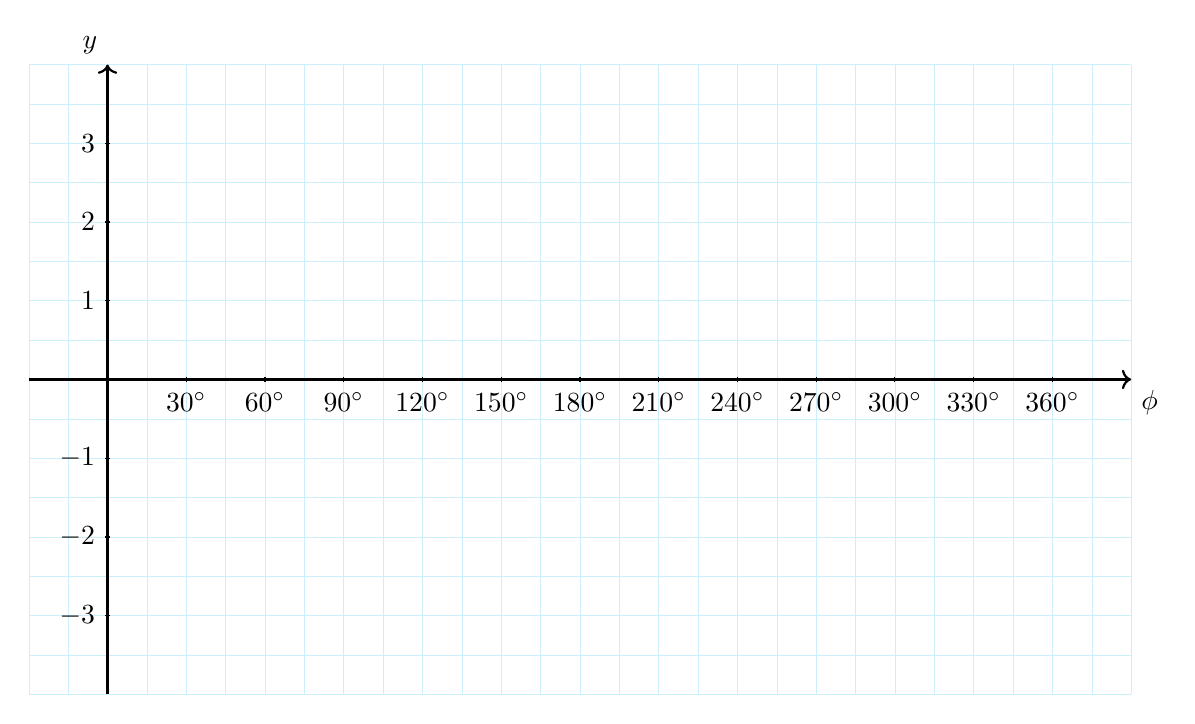
\begin{tikzpicture}
\draw[step = 0.5 cm, cyan!20 , very thin] (-1, -4) grid ( 13, 4);
\draw[thick, ->] (-1,0) -- (13,0) node[anchor = north west] {$\phi$};
\draw[thick, ->] (0,-4) -- (0,4) node[anchor = south east] {$y$};

\foreach \x [evaluate=\x as \degree using int(\x*30)] in {1,...,12}{ 
   \draw (\x cm, 1pt) -- (\x cm, -1pt) node[anchor = north] {$\degree^\circ$};
   }
\foreach \y in {-3,-2,-1,1,2,3}
   \draw (1pt, \y cm) -- (-1pt, \y cm) node[anchor = east] {$\y$};
\end{tikzpicture}}%% END Definition

\newcommand{\trigsysB}{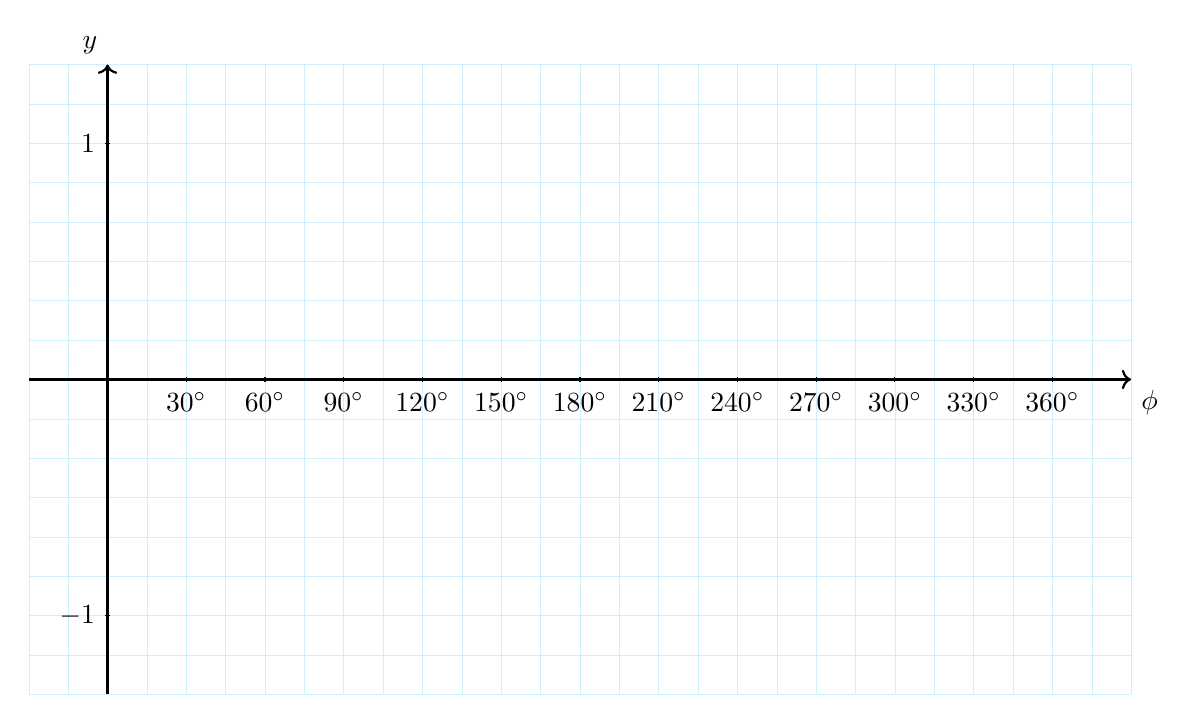
\begin{tikzpicture}\draw[step = 0.5 cm, cyan!20 , very thin] (-1, -4) grid ( 13, 4);
\draw[thick, ->] (-1,0) -- (13,0) node[anchor = north west] {$\phi$};
\draw[thick, ->] (0,-4) -- (0,4) node[anchor = south east] {$y$};

\foreach \x [evaluate=\x as \degree using int(\x*30)] in {1,...,12}{ 
   \draw (\x cm, 1pt) -- (\x cm, -1pt) node[anchor = north] {$\degree^\circ$};
   }
\foreach \y in {-1,1}
   \draw (1pt, \y *3cm) -- (-1pt, \y *3cm) node[anchor = east] {$\y$};

\end{tikzpicture}}%% END Definition

\newcommand{\trigsysC}{
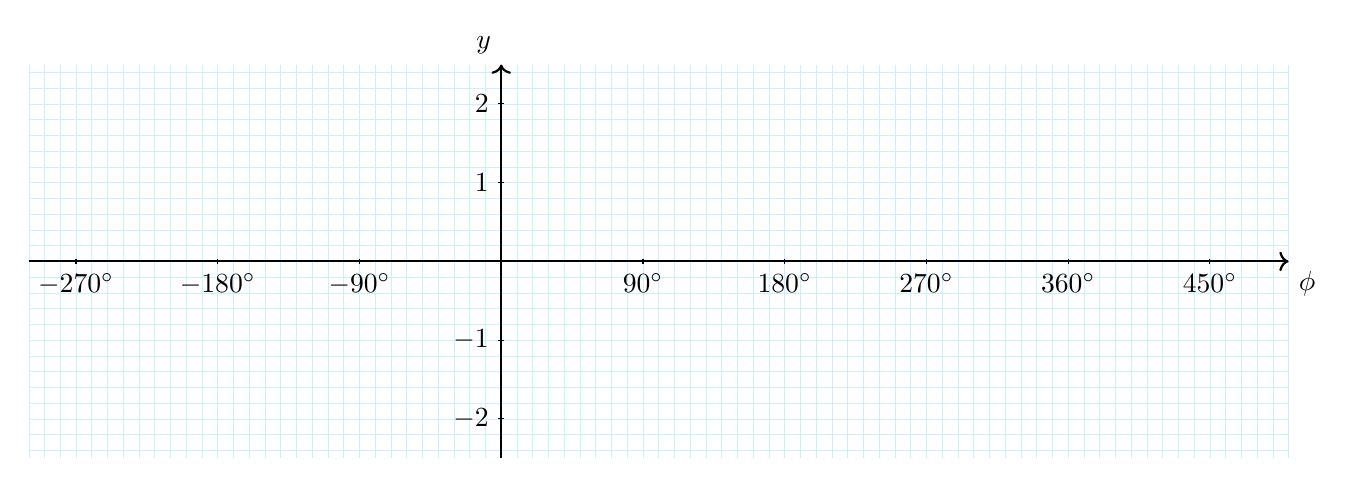
\begin{tikzpicture}
\draw[step = 0.2 cm, very thin, cyan!20] (-6, -2.5) grid ( 10, 2.5);
\draw[thick, ->] (-6,0) -- (10,0) node[anchor = north west] {$\phi$};
\draw[thick, ->] (0,-2.5) -- (0,2.5) node[anchor = south east] {$y$};

\foreach \x [evaluate=\x as \degree using int(\x*90)] in {-3,-2,-1,1,2,3,4,5}{ 
   \draw (\x *18mm, 1pt) -- (\x * 18mm, -1pt) node[anchor = north] {$\degree^\circ$};
   }
   
\foreach \y in {-2,-1,1,2}
   \draw (1pt, \y cm) -- (-1pt, \y cm) node[anchor = east] {$\y$};
\end{tikzpicture}}%% END Definition

\newcommand{\trigsysD}{
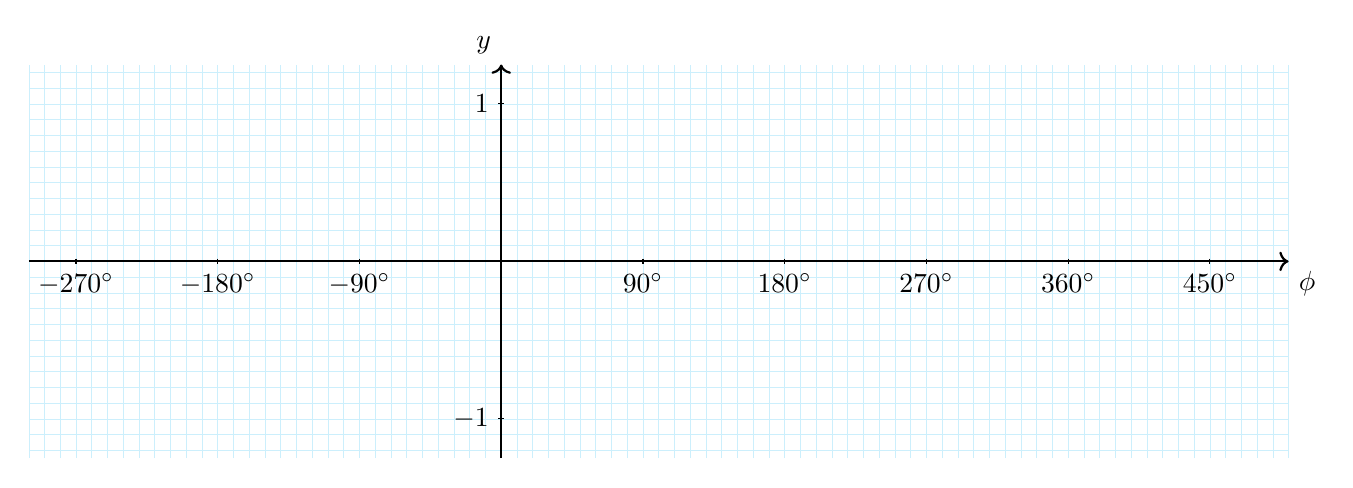
\begin{tikzpicture}
\draw[step = 0.2 cm, very thin, cyan!20] (-6, -2.5) grid ( 10, 2.5);
\draw[thick, ->] (-6,0) -- (10,0) node[anchor = north west] {$\phi$};
\draw[thick, ->] (0,-2.5) -- (0,2.5) node[anchor = south east] {$y$};

\foreach \x [evaluate=\x as \degree using int(\x*90)] in {-3,-2,-1,1,2,3,4,5}{ 
   \draw (\x *18mm, 1pt) -- (\x * 18mm, -1pt) node[anchor = north] {$\degree^\circ$};
   }
   
\foreach \y in {-1,1}
   \draw (1pt, \y *2cm) -- (-1pt, \y *2cm) node[anchor = east] {$\y$};
\end{tikzpicture}}%% END Definition


\newcommand{\trigsysDsin}{
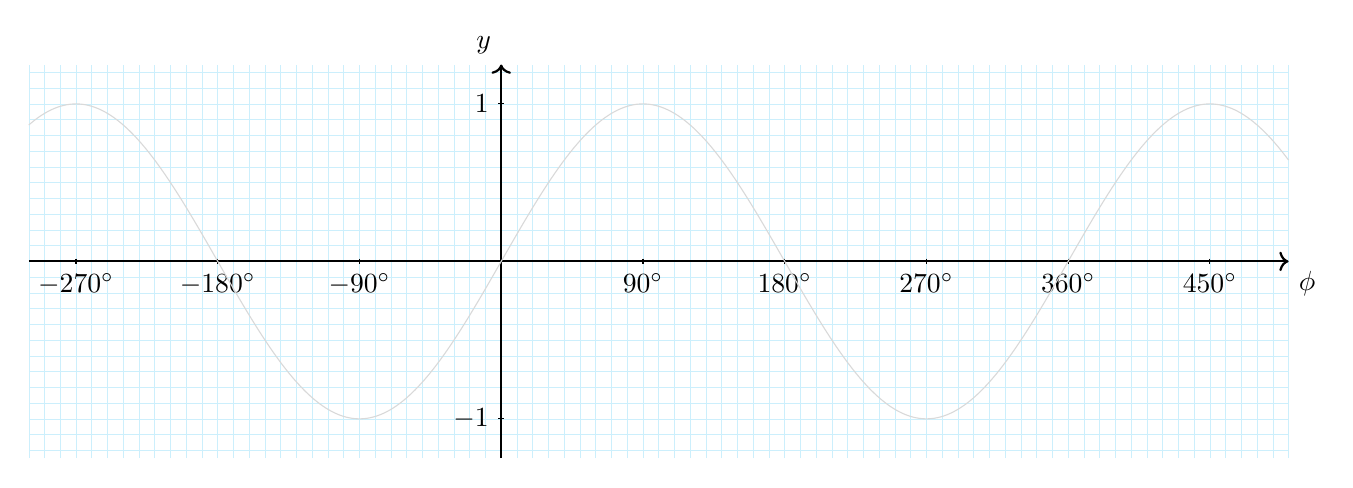
\begin{tikzpicture}
\draw[step = 0.2 cm, very thin, cyan!20] (-6, -2.5) grid ( 10, 2.5);
\draw[thick, ->] (-6,0) -- (10,0) node[anchor = north west] {$\phi$};
\draw[thick, ->] (0,-2.5) -- (0,2.5) node[anchor = south east] {$y$};

\foreach \x [evaluate=\x as \degree using int(\x*90)] in {-3,-2,-1,1,2,3,4,5}{ 
   \draw (\x *18mm, 1pt) -- (\x * 18mm, -1pt) node[anchor = north] {$\degree^\circ$};
   }
   
\foreach \y in {-1,1}
   \draw (1pt, \y *2cm) -- (-1pt, \y *2cm) node[anchor = east] {$\y$};

\draw[domain=-6:10,smooth,samples=200,variable=\x,gray!30] plot ({\x},{2*sin(\x*50)});
\end{tikzpicture}}%% END Definition

\newcommand{\trigsysDcos}{
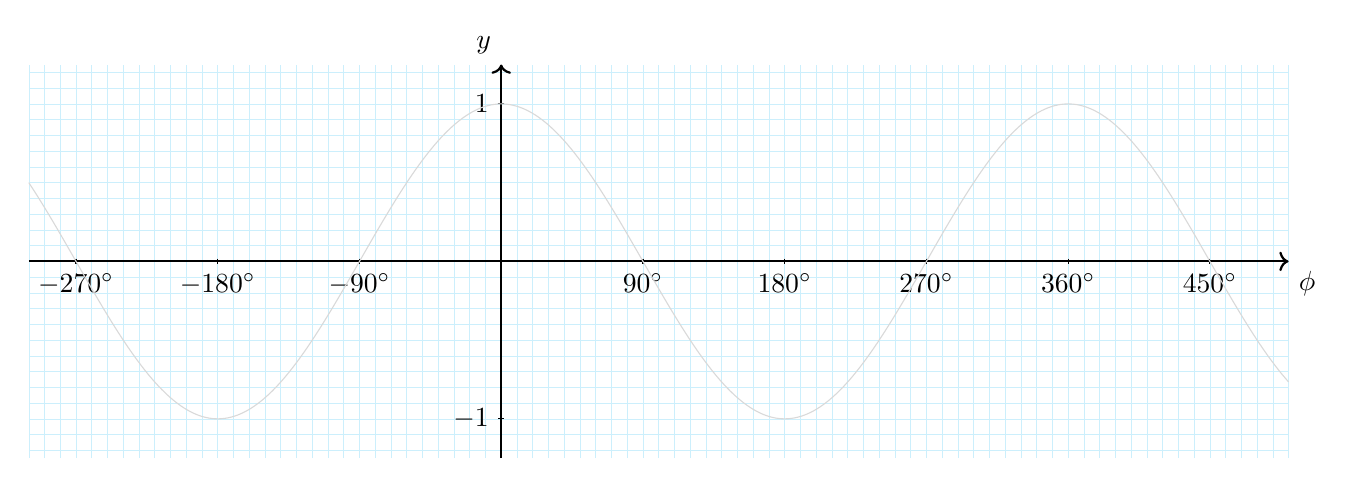
\begin{tikzpicture}
\draw[step = 0.2 cm, very thin, cyan!20] (-6, -2.5) grid ( 10, 2.5);
\draw[thick, ->] (-6,0) -- (10,0) node[anchor = north west] {$\phi$};
\draw[thick, ->] (0,-2.5) -- (0,2.5) node[anchor = south east] {$y$};

\foreach \x [evaluate=\x as \degree using int(\x*90)] in {-3,-2,-1,1,2,3,4,5}{ 
   \draw (\x *18mm, 1pt) -- (\x * 18mm, -1pt) node[anchor = north] {$\degree^\circ$};
   }
   
\foreach \y in {-1,1}
   \draw (1pt, \y *2cm) -- (-1pt, \y *2cm) node[anchor = east] {$\y$};

\draw[domain=-6:10,smooth,samples=200,variable=\x,gray!30] plot ({\x},{2*cos(\x*50)});
\end{tikzpicture}}%% END Definition




\usepackage{bbwLayoutDocSty}

%%%%%%%%%%%%%%%  H E A D E R   &   F O O T E R %%%%%%%%%%%%%%%%%%%%

%% Oben (Header) linke Seite
\fancyhf[HLE]{\makebox{
\includegraphics[width=37mm]{logos/bbwBreit.pdf}}} 
\fancyhf[HCE]{\parttitle}
%% Oben (Header) rechte Seite
\fancyhf[HRO]{\leftmark}
%% Unten (Footer)  FRE = right even, FLE= left even, FRO = right odd,
%% FCO = center odd
\fancyhf[FRE]{\doctitel{}:\ \fachthema}
\fancyhf[FLE,FRO]{\thepage{}/\pageref{LastPage}}
\fancyhf[FCO]{BBW: Abteilung 6 BMS}




\renewcommand{\author}{Philipp G. Freimann}
\renewcommand{\grafikautor}{Ph. G. Freimann}
\renewcommand{\authoremail}{philipp.freimann@bbw.ch}
\renewcommand{\erstellungsdatum}{10. Nov. 2021}
\renewcommand{\docversion}{2.36 \TeX}
\renewcommand{\doctitel}{Denksportaufgaben}

\renewcommand{\fachthema}{Mathematischer Denkanstoß---}
\renewcommand{\ausrichtungAufTitelseite}{}

\begin{document}

\ptitlepage
\newpage

\section{Gefangene}
\subsection{Drei Wächter}
Ein Verließ hat zwei Türen: Die eine führt zur Freiheit, die andere an den
Galgen. Dazwischen stehen drei Wächter. Einer, sagt immer die Wahrheit, einer
lügt immer und der Wankelmütige sagt manchmal die Wahrheit, und manchmal
lügt er. Es ist aber nicht bekannt, wer von den Wächtern welche beschriebene
Eigenschaft hat.
Ein Gefangener darf zwei beliebige Fragen stellen, um herauszufinden, wie er in
die Freiheit gelangt. Jede der beiden Fragen darf jedoch nur einer Person
gestellt werden. Natürlich dürfen beide Fragen auch an dieselbe Person gestellt
werden. Es darf aber keine Frage an mehrere Personen gleichzeitig gestellt
werden.
\TNTeop{}


\subsection{Was muss ein Cracker Fragen, um in die Freiheit zu gelangen?}

Nachdem die acht bekanntesten Cracker endlich gefangen wurden, konnte
ihnen die Schuld dennoch nicht nachgewiesen werden. In dubio pro reo1 hat
sich der Richter gesagt und ihnen am Prozesstag den folgenden Vorschlag
gemacht:

\textit{«Ihr werdet in Einzelhaft gebracht. Jeder in eine eigene Zelle; in einem
Gefängnis mit acht normalen Zellen und einer speziellen Zelle. Ihr werdet keine
Mittel zur Kommunikation untereinander erhalten. Weder Handy, noch sonst
was. Jeden Tag werde ich jedoch irgendeinen von Euch – ganz zufällig – für eine
Stunde in die spezielle Zelle, die Binärzelle sperren. Darin gibt es lediglich einen
Schalter den ihr vom Zustand 0 auf 1 oder vom Zustand 1 auf 0 umschalten
könnt. Dies ist dann auch die einzige Information, die ihr einander hinterlassen
dürft, bevor am nächsten Tag der nächste (oder nach dem Zufallsprinzip wieder
ihr selbst) in die Binärzelle gebracht wird. Nach einigen Wochen werden dann –
ganz nach meinem Auswahlprinzip – alle Acht von Euch einmal in der Binärzelle
gewesen sein. Viele von Euch aber auch mehrfach! Kann mir einer von Euch nun
den Tag nennen, an dem alle mindestens einmal in der Binärzelle waren, dann
seid ihr alle frei. Ihr dürft mir auch später melden und sagen, dass der besagte
Tag nun definitiv vorbei gewesen sei. Ihr müsst also den exakten Tag nicht
angeben können. Wenn ihr es herausfindet, seid ihr alle frei. Meldet ihr es
jedoch zu früh, wird das Verfahren eingestellt und ihr bleibt für den Rest eures
Lebens hinter Gittern. Morgen beginnt das Verfahren, bis dahin könnt ihr noch
beraten, ob ihr darauf eingehen wollt, oder ob ihr gleich für immer hinter Gitter
wollt.»}

Die Cracker beraten sich und nach einiger Zeit kommen sie zum Schluss, dass
sie diesen Vorschlag annehmen wollen. Was haben sie sich wohl für ein
Verfahren ausgedacht, damit sie sicher freikommen?

\TNTeop{}

\newpage
\TRAINER{%% nur Trainerversion
\subsection{Lösungsvorschlag: Drei Wächter}

Die erste Frage des Gefangenen (an einen beliebigen Wächter) lautet: «Welcher
von Deinen Kollegen lügt seltener?»

\begin{itemize}
\item Gerät der Gefangene an den Wahrheitsliebenden, so zeigt dieser diesem
den Wankelmütigen.
\item Gerät er an den Lügner, zeigt dieser auch den Wankelmütigen.
\item Gerät er an den Wankelmütigen, zeigt dieser auf einen der beiden
anderen.
\end{itemize}

In allen drei Fällen aber ist der, auf den nicht gezeigt wird auch nicht der
Wankelmütige.

Diesem dritten kann man der Gefangene also erfolgreich folgende Frage stellen:
«Welchen Weg in die Freiheit würde mir dein Kollege, der das genaue Gegenteil
von dir ist, zeigen?»

\subsection{Lösungsvorschlag: Cracker}
Die Cracker wählen das folgende Verfahren.
Der erste Cracker, der in die Binärzelle geführt wird, wird zum Senior ernannt.
(Also der am ersten Tag ausgewählte.) Der Senior schaltet \textbf{immer}, wenn er in
die Zelle kommt, den Schalter auf 0. Ab seinem zweiten Tag in der Binärzelle
beginnt er mit dem Zählen. Jedes Mal, wenn er in die Zelle kommt und der
Schalter auf 1 ist, zählt der Senior für sich hoch (und schaltet dann den Schalter
sofort wieder auf 0). Wenn er nun sieben Mal hochzählen konnte, meldet er dem
Richter, dass nun alle Gefangenen mindestens einmal in der Binärzelle waren.

Alle anderen Cracker verfahren wie folgt. Sie dürfen während der ganzen
Gefangenschaft den Schalter in der Binärzellen nur ein einziges Mal von 0 auf 1
umschalten. Kommen sie in die Binärzelle und der Schalter ist bereits auf 1,
dann tun sie gar nichts. Das bedeutet nämlich, dass ein Gefangener vor ihnen
bereits seinen «Zähler» verbraucht hat. Kommen sie jedoch in die Zelle und der
Schalter ist auf 0, so können sie nun den Schalter auf 1 umlegen. Dies dürfen sie
aber, wie erwähnt, während der ganzen Gefangenschaft nur ein einziges Mal
tun. Dieses umlegen zählt nämlich ihren eigenen Besuch in der Binärzelle.

Hat der Senior nun auf 7 gezählt, so ist jeder der anderen Gefangenen bereits
einmal in der Zelle gewesen und der Senior kann dem Richter melden, dass der
Zeitpunkt der Freilassung nun endlich gekommen sei.
Zusatzaufgabe: Programmieren Sie dieses Verfahren, um herauszufinden, wie
lange es im Durchschnitt braucht, bis die acht Cracker frei sind.
}%% END TRAINER Lösungsvorschlag
\newpage


\section{Zwei Eimer}
Vor einem Brunnen stehen zwei Eimer. Diese weisen keinerlei Markierungen
auf. Einer der Eimer fasst 5 Liter, der andere fasst 7 Liter. Ziel ist es, einen (1)
Liter abzumessen.

Wie ist vorzugehen? Wer findet die Lösung, bei der am wenigsten umzuschütten
ist?
\TNTeop{}
\TRAINER{%% Lösungsvorschlag nur Trainer}
\subsection{Lösungsvorschlag: Zwei Eimer}

\begin{enumerate}
\item
Beide Eimer leeren.
\item
5 Liter abmessen und
\item
in den (leeren) 7-Liter-Eimer füllen.
\item
5 Liter abmessen
\item
und 2 Liter in den 7-Liter-Eimer füllen. Es bleiben 3 Liter im 5-Liter-
Eimer.
\item
7-Liter-Eimer leeren.
\item
Die 3 Liter aus dem 5-Liter-Eimer in den (leeren) 7-Liter-Eimer einfüllen.
\item
5-Liter-Eimer ganz auffüllen.
\item
4 Liter aus dem 5-Liter-Eimer in den 7-Liter-Eimer einfüllen (der ist jetzt
voll); im 5-Liter-Eimer bleibt genau ein Liter übrig.
\end{enumerate}

Andere Variante:
\begin{enumerate}
\item
Beide Eimer leeren.
\item
7 Liter abmessen
\item
in den (leeren) 5-Liter-Eimer füllen. Es bleiben 2 Liter im 7-Liter-Eimer.
\item
5-Liter-Eimer ausleeren.
\item
2 Liter aus dem 7-Liter-Eimer in den 5-Liter-Eimer umfüllen.
\item
7-Liter-Eimer neu füllen.
\item
3 Liter aus dem 7-Liter-Eimer in den 5-Liter-Eimer umfüllen (mehr hat im
5-Liter-Eimer nicht Platz).
\item
5-Liter-Eimer ausleeren.
\item
Die 4 verbleibenden Liter aus dem 7-Liter-Eimer in den 5-Liter-Eimer
einfüllen.
\item
7-Liter-Eimer wieder auffüllen.
\item
Ein Liter aus dem 7-Liter-Eimer in den 5-Liter-Eimer einfüllen (es bleiben
6 Liter im 7-Liter-Eimer).
\item 
5-Liter-Eimer entleeren.
\item
5 Liter aus dem 7-Liter-Eimer in den 5-Liter-Eimer füllen. Es bleibt ein
Liter im 7-Liter-Eimer.
\end{enumerate}

}%% END TRAINER
\newpage
\section{Zahlen}
\subsection{Französischer Spion}
Im Deutsch-Französischen Krieg 1870/71 will ein französischer Spion
unbemerkt in eine deutsche Stadt gelangen. Die Stadt hat eine Schutzmauer
und wird von einem Wächter bewacht. Der Franzose versteckt sich in einem
Gebüsch und versucht herauszufinden, wie die Stadtbewohner an der Wache
vorbeikommen.

Zuerst kommt ein Bauer und der Wächter ruft fragend «8 . Der Bauer antwortet
«4» und wird hineingelassen. Jetzt kommt eine Nonne und wird vom Wächter
gefragt: «16»? Sie antwortet «8» und wird ebenfalls eingelassen. Jetzt kommt ein
Mönch. Der Wächter fragt nach «28». Der Mönch antwortet «14». Auch er kann
passieren.

Jetzt glaubt unser Französische Spion das Spiel durchschaut zu haben und geht
auf das Stadttor zu. Er wird vom Wächter nach «14» gefragt, antwortet mit «7»
und wird noch am selben Tage exekutiert.

Was hätte er auf die Frage des Wächters antworten sollen?

\subsection{Falsche Rechnungen?}
In dieselbe Kategorie geht die Aufgabe, die mir ein Kursteilnehmer per E-Mail
zur Verfügung gestellt hat.

8890 = 6

6633 = 2

7722 = 0 

7563 = 1

7387 = 2

1838 = 4

7237 = 0
 
5656 = 2

8398 = 5

1386 = ???

\TNTeop{}

\TRAINER{%%
\subsection{Lösungsvorschlag: Spion}
Die Zahlen sind als Text zu lesen und nicht als Zahlenwerte oder Ziffernfolge.
Die Zahl „acht“ hat 4 Buchstaben.

„Sechzehn“ hat 8 Buchstaben.

„Achtundzwanzig“ hat 14 Buchstaben.

Somit hätte der Spion auf die Frage „14“ einfach 8 antworten sollen.

\subsection{Lösungsvorschlag: Falsche Rechnungen}

Zählen Sie einfach die Anzahl der geschlossenen Kreise. 6, 9 und 0 besitzen je
einen Kreis, 8 besitzt 2 Kreise. (Die Aufgabe kann am besten von
Vorschulkindern gelöst werden.)

Lösung 1386 = 3
}%% END TRAINER

\newpage

\section{Wiegeprobleme}
\subsection{König}



Der König treibt im ganzen Land die Steuern ein. Jeder der 100 Bürger muss
einen Sack mit 1000 Goldmünzen abliefern. Dem König wird bekannt, dass unter
den Bürgern ein Betrüger ist, dessen Goldmünzen gefälscht sind. Seine Münzen
sind rein optisch von den anderen nicht zu unterscheiden, wiegen aber nur 9g,
anstelle der gewöhnlichen 10g.

Wie kann der König mit nur einem
Wiegevorgang den Betrüger herausfinden?

Bemerkung: Der König hat eine sehr
genaue Waage, die jedoch nur ein einziges Mal funktioniert.

\TNTeop{}

\subsection{Karamell}
Der Besitzer eines Krämerladens möchte Zucker pfundweise von einem bis zu
40 Pfund abwiegen können. Er hat nur eine altmodische Waage zur Verfügung,
bei der die abzuwiegende Menge in einer Waagschale mit den entsprechenden
Gewichten in der anderen Schale ausbalanciert wird. Da er ein effizienter und
sparsamer Mann ist, will er sich nur so viele Gewichte besorgen, wie unbedingt
nötig sind, um jede Menge von einem bis zu 40 Pfund in einem einzigen
Wiegevorgang abzuwiegen.

a) Wie viele Gewichte benötigt er und wie groß sind sie, wenn sie nur auf einer
Seite der Waage benutzt werden dürfen?

b) Wie viele Gewichte sind nur noch nötig, wenn er Gewichte auf beide Schalen
legen darf?
\TNTeop{}

\TRAINER{%%
\subsection{Lösungsvorschlag: König}

Der König nimmt vom ersten Sack 1 Münze, vom zweiten Sack 2 Münzen, vom
dritten Sack 3 Münzen, usw. heraus. Bei 100 Säcken hat er 5050 Münzen
herausgenommen, die somit (unterstellt keine sei gefälscht) 50.500g wiegen
müssten. Beträgt sein Wiegeergebnis allerdings beispielsweise 34g weniger, so
weiß er, dass der Bürger, dem er 34 Münzen aus dem Sack genommen hat der
Betrüger ist! Denn seine Münzen sind ja 1g leichter.

Quelle: \texttt{www.denksport-ecke.de}


\subsection{Lösungsvorschlag: Karamell}

(Quelle: Paul Sloane: Neue Denkpuzzles für helle Köpfe):
Tipp: Ob Sie’s glauben oder nicht, es ist tatsächlich möglich, jedes beliebige
Gewicht zwischen einem und 40 Pfund mit nur vier verschiedenen Gewichten
abzuwiegen. Das setzt allerdings voraus, dass es erlaubt ist, die Gewichte in
beide Waagschalen zu legen (Aufgabe b). Wenn Sie nur eine Waagschale für die
Gewichte benutzen dürfen (Aufgabe a), dann brauchen Sie insgesamt 6
Gewichte. Doch damit können Sie dann alle Gewichte von einem bis 63 Pfund
bestimmen.

a) Die Gewichte haben die Massen 1, 2, 2, 5, 10 und 20 Pfund. Alternativ: 1, 2,
4, 8, 16 und 32 Pfund. Vorteil der 1. Variante: Gängige Zahlen sind einfacher zu
berechnen. Vorteil 2. Variante: Sogar Gewichte bis zu 63 Pfund sind alle
abmessbar.

b) Die Massen betragen: 1, 3, 9 und 27 Pfund.
Um Beispielsweise 16 Pfund abzuwiegen, legt der Kramer 28 (27 + 1) Pfund auf
die eine Schale und 12 (9 + 3) Pfund auf die andere Schale: 28 – 12 ergibt 16
Pfund: so braucht er nur noch 16 Pfund Zucker auf die zweite Schale zu kippen
und die Waage ist im Gleichgewicht.
}%% END TRAINER
\newpage

\section{Prozentrechnungen}


\begin{center}\textit{«125\% der Leute können nicht Bruchrechnen. Das ist jeder vierte, nein mehr
noch: jeder fünfte!»}\end{center}


\subsection{Skonto}

Beim Kauf ab zwei Artikeln gewährt der Verkäufer 5\% Rabatt. Bei einer
Barzahlung gewährt er zusätzlich 3\% Skonto. Ist es nun schlauer, das Skonto
zuerst einzufordern und dann die 5\% Rabatt oder besser zuerst die 5\% Rabatt
und dann die 3\% Skonto?

\TNTeop{}

\subsection{Gemüse}
Ein Früchte- und Gemüsehändler hatte eine Tonne (1000kg) Gemüse (z. B.
Gurken) geerntet. Seine Messung hatte ergeben, dass die Ware zu 98\%\,
(Gewichtsprozente) aus Wasser besteht.
Leider konnte er das Gemüse auf dem Markt nicht sofort verkaufen, sodass es
einige Tage liegen blieb. Als er es endlich verkaufen kann, ergibt die Messung,
dass die Ware nur noch einen Wasseranteil von 95\% aufweist.
Wie schwer ist die Ware nun?

\TNTeop{}

\subsection{Umsatzsteigerung}
Ein Händler gibt neu einen Rabatt von 10\% auf sein Sortiment. Laut
Branchenverband müsste der Händler nun 70\% mehr Umsatz\footnote{Umsatz = Einnahmen durch Verkauf der Ware, also Einkaufspreis + Marge.} 1 machen, wie vor
der Reduktion, um den ursprünglichen Gewinn zu erzielen.
Reichen diese Angaben, um die ursprüngliche Marge\footnote{Marge = Differenz von Einkaufspreis zum Verkaufspreis; m. a. W. der gesuchte
Gewinn.} 2 zu bestimmen?

\TNTeop{}


\TRAINER{%%
\subsection{Lösungsvorschlag: Skonto}

Die Reihenfolge spielt keine Rolle, es sei denn, es werde zwischen den beiden
Abzügen auf- oder abgerundet. Begründung: 5\% Rabatt entspricht einer
Multiplikation mit Faktor 0.95; 3\% Skonto entspricht einem Faktor 0.97. Nun
gilt aber
(Preis * 0.95) * 0.97 = (Preis * 0.97) * 0.95 (Kommutativgesetz) = 0.9515
Noch besser wäre es, vom Verkäufer direkt 8\% einzufordern, sofern er damit
einverstanden wäre ;-)

5.5. Lösungsvorschlag: Prozentrechnung
Der einfachste Weg geht hier über den festen Bestandteil des Gemüses. Die
erste Messung ergibt einen Wasseranteil von 98\%, das bedeutet, dass das
Gemüse anfänglich einen Anteil von 980kg Wasser enthält: lediglich 20kg sind
kein Wasser (also fester Bestandteil).
Die zweite Messung ergibt einen Wasseranteil von 95\%. Das bedeutet aber, dass
5\% fester Anteil sind. 5\% sind aber die 20kg aus der ersten Messung. Die
Festbestandteile haben sich ja nicht geändert. Nun lautet die Aufgabe viel
einfacher: 20kg entsprechen 5\%, wie viel sind 100%?
Die einfache aber doch noch etwas verblüffende Antwort lautet: 400kg (wovon
380kg Wasser sind.)
Man könnte sich nun fragen: „Was(?), eine Abnahme von 3\% Wasser macht
600kg aus?“ Das wäre natürlich falsch. Es werden ja eben nicht einfach 3\% des
Wassers entzogen, sondern das Verhältnis Wasser zu Festbestandteil ändert
sich um 3\%.
\newpage

\subsection{Lösungsvorschlag: Umsatzsteigerung}

\textbf{Zeitpunkt 1 (vor dem Abschlag):}

Einkaufspreis Ware vorher = EP1 = 100% = 1 (z. B. 100.- CHF)
$$m = \text{(Aufschlags)Marge (als Faktor) vor dem Abschlag}$$
$$\text{Verkaufspreis ursprünglich} = EP \cdot{} (1+m) = 1+m,$$
da ich EP auf eine Einheit (EP) gesetzt hatte (\zB $100.- \cdot{} (1+m)$)


\textbf{Zeitpunkt 2 (nach dem Abschlag, aber vor der Umsatzsteigerung):}

$(1+m)\cdot{}0.9$ = Verkaufspreis nach dem Abschlag (vor der Umsatzsteigerung)

$y := (1+m)\cdot{}0.9 - 1 =$ Marge nach der Reduktion (als Faktor z. B. 0.15 o. ä.)

\textbf{Zeitpunkt 3 (nach der Umsatzsteigerung gegenüber Zeitpunkt 1):}

$1.7(1+m)$ = Umsatzsteigerung gegenüber ursprünglichem Umsatz


$x :=$ Zunahme im Einkauf (unbekannt) (als Faktor gegenüber dem ursprünglichen Einkaufspreis)

$xy =$ Gewinnzunahme gegenüber dem Gewinn aus Zeitpunkt 2.

$1+x = $neuer Einkauf (genau $EP \cdot{} (1+x)$)

$1+y + x + xy =$ neuer Umsatz (Genau genommen $EP \cdot{} (1+y) + x\cdot{}EP \cdot{}(1+y)$,
daher das $xy$)

$y+xy = $neuer Gewinn (und dieser muss ja gleich der alten Marge sein $(y+xy=m)$)
Der neue Umsatz muss nun gleich 170\% des ursprünglichen Umsatzes sein.

Ergo:

$$\Longrightarrow 1+x+y+xy = 1.7(1+m)$$

Die drei Gleichungen nun so (1:1) in \texttt{wolframalpha.com} eintragen:

wolframalpha.com -> $$\{ y=9*(1+m)/10-1, y+xy=m, 1+x+y+xy=17*(1+m)/10\}$$

(die 2. Lösung $m=-1$, also die Marge = -100\% vor der Reduktion ist hier zu
vernachlässigen, das würde bedeuten, er habe die Ware immer gratis
abgegeben.)

Frei nach Wolframalpha:

* Ursprüngliche (Aufschlags)Marge: \textbf{17/63}

* Neue (Aufschlags)Marge: 1/7

* Einkaufszuname: 8/9

PS: Natürlich müssen wir die Resultate an einem Zahlenbeispiel noch
nachrechnen; also eine Probe machen, ob die Resultate sinnvoll sind.
Das Gleichungssystem nicht von Hand ausrechnen: a) geht zu lange b) ist
fehleranfällig.
\newpage
}%% end TRAINER


\section{Alter}
\subsection{Petra und Anton}

Petra ist jetzt 24 Jahre alt. Sie ist doppelt so alt wie Anton war, als Petra so alt
war, wie Anton jetzt ist.

Wie alt ist Anton?


\subsection{Du und ich}

Als du so alt warst wie ich heute bin, warst du dreimal so alt wie ich. Und wenn
ich dreimal so alt sein werde wie ich heute bin, dann sind wir zusammen genau
ein Jahrhundert alt.

Wie alt bin ich? Wie alt bist Du?


\subsection{Aus einer Mathematikolympiade (Singapur)}
Alice und Bob haben Zegna kennen gelernt und wollen ihren Geburtstag wissen.
Zegna nennt den beiden zehn mögliche Daten:

15. Mai, 16. Mai, 19. Mai,

17. Juni, 18. Juni,

14. Juli, 16. Juli,

14. August, 15. August und 17. August.



Zegna verrät Alice nur den Geburtsmonat und Bob nur den Tag. Dann sprechen
die beiden miteinander.

Alice sagt zu Bob: «Ich weiß nicht, wann Zegna Geburtstag hat, aber ich weiß,
dass Du es auch nicht weißt.»

Darauf erwidert Bob: «Zu Anfang wusste ich auch nicht, wann Zegna Geburtstag
hat, aber jetzt, dank Deiner Information, weiß ich es.»

Alice: «Jetzt kenne ich ihren Geburtstag auch.»

Wann hat Zegna Geburtstag?
\TNTeop{}


\subsection{Wo ist der Vater?}

Die Mutter ist um 21 Jahre älter als ihr Kind. In sechs Jahren wird dann die
Mutter fünf mal so alt sein wie das Kind. Wo ist der Vater jetzt?

\TNTeop{}

\TRAINER{
\subsection{Lösungsvorschlag: Anton und Petra}

Anton ist 18. Damals in der Vergangenheit, war er halb so alt, also 12 Jahre.
Petra war aber damals gleich alt, wie Anton heute ist:

\begin{tabular}{|c|c|c|}\hline
 & Petra & Anton\\\hline
 Vergangenheit (war) & $x$ & 12 \\\hline
 Gegenwart (ist) & 24 & $x$\\\hline
 \end{tabular}

Die Differenz von $x$ bis 24 muss aber gleich groß sein, wie die Differenz von 12
zu $x$.

In Formeln: $24-x = x - 12$ woraus folgt, dass $x = 18$.
 

\subsection{Lösungsvorschlag: Ich und Du}

Wieder kann die Lösung mit einer Tabelle einfach gefunden werden:

\begin{tabular}{|c|c|c|}\hline
 & du &  ich \\\hline
war (Vergangenheit) & $3x$ & $x$ \\\hline
ist (Gegenwart) & $5x$ & $3x$  \\\hline
sein wird (Zukunft) & $11x$ & $9x$\\\hline
 \end{tabular}
 
11X + 9X = 100 woraus folgt, dass X = 5 ist. \textbf{«Ich bin 15, du bist 25»}

\newpage

\subsection{Lösungsvorschlag: Mathematikolympiade}

\begin{tabular}{|c|c|c|c|c|c|c|}\hline
       & 14. & 15. & 16. & 17. & 18. & 19.\\\hline

Mai    &     & 1.  & 1.     &     &     & 1. \\\hline
Juni   &     &     &        & 1.  & 1.  &  \\\hline
Juli   &  2. &     & Lösung &     &     & \\ \hline
August & 2.  & 2.  &        & 3.  &     & \\\hline
 \end{tabular}

1.: Mai und Juni fallen weg, ansonsten wüsste Alice nicht, ob es Bob weiß (18.
Juni und 19. Mai wären eindeutig für Bob).

2.: Nun weiß es Bob, somit fällt der 14. weg.

3.: Da es Alice schlussendlich weiß, fällt der August weg.


\subsection{Lösungsvorschlag: Wo ist der Vater?}

Nach dem Lösen der Gleichung [$(x+21)+6 = 5·(x+6)$; $x$ = Alter des Kindes
heute] erhalten wir, dass das Kind heute genau $-\frac34$ Jahre, also minus neun
Monate alt ist.

}%% END Trainer





\end{document}


